\documentclass[12pt, openany]{report}
\usepackage[utf8]{inputenc}
\usepackage[T1]{fontenc}
\usepackage{amsmath,amsfonts,amssymb}
\usepackage{amssymb}
\usepackage{multicol}
\usepackage[a4paper,left=2.5cm,right=2.5cm,top=2.5cm,bottom=2.5cm]{geometry}
\usepackage[french]{babel}
\usepackage{libertine}
\usepackage{graphicx}
\usepackage{wrapfig}
\usepackage{algorithm}
\usepackage{algpseudocode}
\usepackage{float}
\usepackage{enumitem}
\usepackage{pythonhighlight}
\usepackage[]{titletoc}
\usepackage{empheq}
\usepackage{titlesec}
\usepackage{mathpazo}
\usepackage{xfrac}
\usepackage{textcomp}
\usepackage{mathtools}
\usepackage{caption}
\usepackage{tabularray}
\usepackage{subcaption}
\usepackage[bottom]{footmisc}
\usepackage{pdfpages}
\usepackage{tabularx}
\usepackage{amsthm}
\usepackage[skins]{tcolorbox}
\titleformat{\chapter}[display]
  {\normalfont\bfseries}{}{0pt}{\Huge}
\usepackage{hyperref}
\newcommand{\hsp}{\hspace{20pt}}
\newcommand{\HRule}{\rule{\linewidth}{0.5mm}}
\newcommand{\R}{\mathbb{R}}
\newcommand\independent{\protect\mathpalette{\protect\independenT}{\perp}}
\def\independenT#1#2{\mathrel{\rlap{$#1#2$}\mkern2mu{#1#2}}}

% Define a new tcolorbox style with a red border and transparent interior
\tcbset{
    redbox/.style={
        enhanced,
        colframe=red,
        colback=white,
        boxrule=1pt,
        sharp corners,
        before skip=10pt,
        after skip=10pt,
        box align=center,
        width=\linewidth-2pt, % Adjust the width dynamically
    }
}
\newcommand{\boxedeq}[1]{
\begin{tcolorbox}[redbox]
    \begin{align}
        #1
    \end{align}
\end{tcolorbox}
}
\theoremstyle{definition}
\newtheorem{thm}{Theorem}[chapter]
\newtheorem{definition}[thm]{Definition}
\newtheorem{exmp}[thm]{Example} 
\newtheorem{lem}[thm]{Lemma}
\newtheorem{prop}[thm]{Property}
\newtheorem{crl}[thm]{Corollary}
\begin{document}


\begin{titlepage}
    \begin{sffamily}
    \begin{center}
        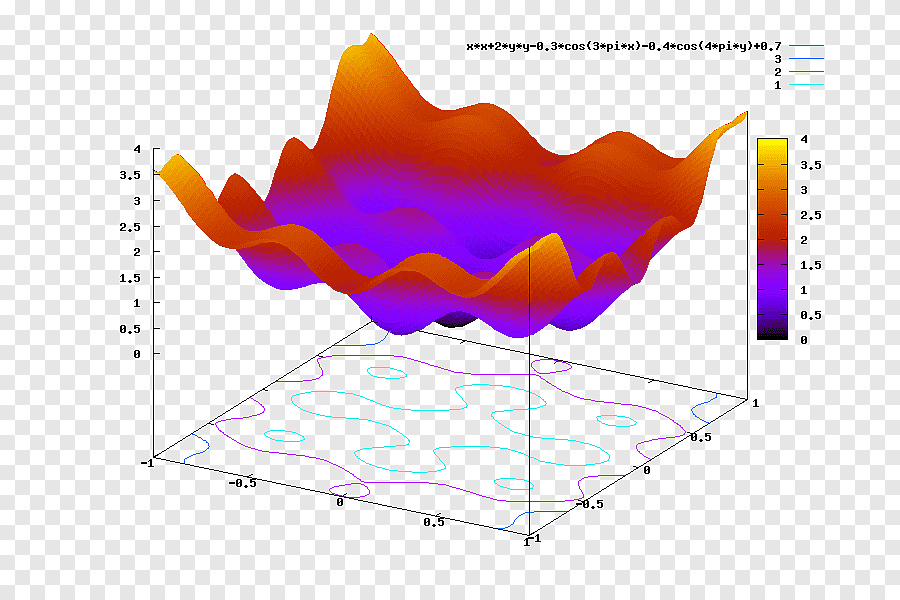
\includegraphics[scale=0.25]{img/page_de_garde.png} \\[1cm]
        \HRule \\[0.4cm]
        { \huge \bfseries LINMA2471 Optimization models and methods II \\[0.4cm] }
    
        \HRule \\[1.5cm]
        \textsc{\LARGE Simon Desmidt}\\[1cm]
        \vfill
        \vspace{2cm}
        {\large Academic year 2024-2025 - Q1}
        \vspace{0.4cm}
         
        
\includegraphics[width=0.15\textwidth]{img/epl.png}
        
        UCLouvain\\
    
    \end{center}
    \end{sffamily}
\end{titlepage}

\setcounter{tocdepth}{1}
\tableofcontents
\chapter{Gradient Method}
An optimization problem is defined as 
\begin{equation}\label{eq:1}
    \min_{x\in \mathbb{R}^n} f(x)
\end{equation}
where \(f:\mathbb{R}^n\rightarrow\mathbb{R}\) is a continuously differentiable function. 
\section{Definitions}
\begin{itemize}
    \item A function \(F:\mathbb{R}^n\rightarrow \mathbb{R}^n\) is L-Lipschitz continuous when \[\lVert F(y)-F(x)\rVert \le L\lVert y-x\rVert\qquad \forall x,y\in \mathbb{R}^n\]where we use the euclidian norm. 
    \item If \(\nabla f\) is L-Lipschitz then, given \(x\in \mathbb{R}^n\), \[f(y)\le f(x)+\langle \nabla f(x), y-x\rangle +\frac{L}{2}\lVert y-x\rVert^2 = m_x(y)\qquad \forall y\in \mathbb{R}^n\]and \(f\) is said to be a L-smooth function.
    \item We say that a differentiable function \(\Psi:\mathbb{R}^n\rightarrow \mathbb{R}\) is L-smooth for some \(L\ge 0\) when, given \(x\in \mathbb{R}^n\), \[\Psi(y) \le \Psi(x) + \langle \nabla \Psi (x),y-x\rangle + \frac{L}{2}\lVert y-x\rVert^2 \qquad \forall y\in \mathbb{R}^n\]
    \item A convex function \(f:\mathbb{R}^n \rightarrow \mathbb{R}\) is convex when, given \(x,y\in \mathbb{R}^n\) and \(\lambda \in [0,1]\), we have \[f(\lambda x+(1-\lambda)y)\le \lambda f(x)+(1-\lambda)f(y)\]
    \item Let \(f:\mathbb{R}^n\rightarrow\mathbb{R}\) be convex. If \(f\) is differentiable, then \[f(y) \ge f(x) + \nabla f(x)^T (x-y) \qquad \forall x,y\in \mathbb{R}^n\]
    \item A differentiable function \(f:\mathbb{R}^n\rightarrow \mathbb{R}\) is \(\mu\)-strongly convex \((\mu>0)\) if, given \(x\in \mathbb{R}^n\), \[f(y) \ge f(x) + \nabla f(x)^T(y-x) + \frac{\mu}{2}\lVert y-x\rVert^2 \qquad \forall y\in \mathbb{R}^n\]
    \item PL inequality for a \(\mu\)-strongly convex function\footnote{\(x^*\) is the minimizer of \(f\)}: \[f(x)-f(x^*)\le \frac{1}{2\mu} \lVert \nabla f(x)\rVert^2 \qquad \forall x\in \mathbb{R}^n\]
\end{itemize}
\section{Complexity}
The demonstration of the final results here obtained is in the notes, but not explained here. 
\subsection{Hypotheses}
\begin{itemize}
    \item \(f\) is convex and differentiable;
    \item \(\nabla f\) is L-Lipschitz;
    \item we start from a \(x_0\in \mathbb{R}^n\) that is not a minimizer of \(f\);
\end{itemize}
\subsection{Results}
We use the sequence \(\{x_k\}_{k\ge 0}\), given a \(x_0\in \mathbb{R}^n\), such that \[x_{k+1} = x_k - \frac{1}{L}\nabla f(x_k)\]
\begin{center}
    \renewcommand{\arraystretch}{1.5}
    \begin{tabular}{c|c|c}\label{tab:complexity}
    Problem class & Goal & Complexity bound \\ \hline\hline
    Non-convex \(f\) & \(\lVert \nabla f(x_k)\rVert \le \varepsilon\) & \(\mathcal{O}(\varepsilon^{-2})\)\\ \hline
    Convex \(f\) & \(f(x_k)-f(x^*)\le \varepsilon\) & \(\mathcal{O}(\varepsilon^{-1})\)\\ \hline
    \(\mu\)-strongly-convex \(f\) & \(f(x_k)-f(x^*)\le \varepsilon\) & \(\mathcal{O}(\log (\varepsilon^{-1}))\)
\end{tabular}
\end{center}
\section{GM with Armijo Line Search}\label{sec:armijo}
The Armijo Line Search consists of changing the constant in the GM in order to be more efficient and be able to make bigger steps in some directions where it is possible. 
\begin{equation}
    x_{k+1} = x_k - \alpha \nabla f(x_k)\qquad \alpha >0
\end{equation}
\begin{algorithm}
    \caption{Gradient Method with Armijo Line Search}\label{algo:Armijo}
    \begin{algorithmic}[1]
    \State \textbf{Step 0:} Given $x_0 \in \mathbb{R}^n$ and $\alpha_0 > 0$, set $k \coloneqq 0$.
    \State \textbf{Step 1:} Set $\ell \coloneqq 0$.
    \State \textbf{Step 1.1:} Compute $x_k^+ = x_k - (0.5)^\ell \alpha_k \nabla f(x_k)$.
    \State \textbf{Step 1.2 (Armijo Line Search):} If
    \[
    f(x_k) - f(x_k^+) \geq \frac{(0.5)^\ell \alpha_k}{2} \|\nabla f(x_k)\|^2 \tag{1}
    \]
    set $\ell_k \coloneqq \ell$ and go to Step 2. Otherwise, set $\ell \coloneqq \ell + 1$ and go back to Step 1.1.
    \State \textbf{Step 3:} Define $x_{k+1} = x_k^+$, $\alpha_{k+1} = (0.5)^{\ell_k - 1} \alpha_k$, set $k \coloneqq k + 1$ and go back to Step 1.
    \end{algorithmic}
\end{algorithm}
\section{Problems with convex constraints}
Consider the problem
\begin{equation}\label{eq:convex_problem}
    \min_{x\in \mathbb{R}^n} f(x) \text{ such that } x\in \Omega
\end{equation}
where \(f\) is L-smooth, and \(\Omega \subseteq \mathbb{R}^n\) is nonempty, closed and convex.
Given an approximation \(x_k\in \Omega\) for a solution of \ref{eq:convex_problem}, a possible generalization of the Gradient Method is to define 
\begin{equation}
    x_{k+1} = P_{\Omega} \left(x_k-\frac{1}{L}\nabla f(x_k)\right)
\end{equation}
where \(P_{\Omega}\) is the projection of \(z\) onto \(\Omega\), and we call this method the Projected Gradient Method.\\
If \(\Omega = [a,b]^n\), then the projection of an element \(z\) onto \(\Omega\) is such that its element \(i\) is given by:
\begin{equation}
    \left[P_\Omega(z)\right]_i = \begin{cases}
        z_i \text{ if } a\le z_i\le b\\
        a \text{ if } z_i<a\\
        b \text{ if }z_i>b\\
    \end{cases} \qquad \forall i=1,\dots,n
\end{equation}
If \(x^*\) is a solution of \eqref{eq:convex_problem}, then \[\langle \nabla f(x^*),z-x^*\rangle \ge 0\qquad \forall z \in \Omega\]
\begin{itemize}
    \item [\(\rightarrow\)] Note: if \(\Omega = \mathbb{R}^n\), then this lemma is true, in particular for \(z=x^*-\nabla f(x^*)\). Then it is straightforward that we must have \(\nabla f(x^*)=0\). 
\end{itemize}
\section{Reduced gradient method}
For a L-smooth function for the problem \eqref{eq:convex_problem}, we define 
\begin{equation}
    G_L(x_k) = L(x_k-x_{k+1})
\end{equation}
where \(x_{k+1}\) is given by the general formula\footnote{This definition of \(x_{k+1}\) is true for any type of gradient method, the first case seen being with \(\Omega = \mathbb{R}^n\).}
\begin{equation}
    x_{k+1} = \arg \min_{y\in \Omega} f(x_k) + \langle \nabla f(x_k),y-x_k\rangle +\frac{L}{2}\lvert y-x_k\rVert_2^2
\end{equation}
From this, we can show as we did in the previous sections that there is a lower bound for the method:
\begin{equation}
    f(x_k)-f(x_{k+1}) \ge \frac{1}{2L}\lVert G_L(x_k)\rVert_2^2
\end{equation}
This is the same result we found for the unconstrained gradient method, but with a different gradient definition. This is thus a generalization of the first cases. Furtheremore, by the same process we used before, we can show that the complexity of this Reduced Gradient Method is the same as in the table \ref{tab:complexity}.
\section{Proximal Gradient Method}
We will here consider problems of the form 
\begin{equation}
    \min_{x\in \mathbb{R}^n} F(x) \equiv f(x) + \phi(x)
\end{equation}
where \(f(\cdot)\) is L-smooth and \(\phi :\mathbb{R}^n\rightarrow \mathbb{R}\cup \{+\infty\}\) is convex, possibly nonsmooth. \\
In this case, the formula for \(x_{k+1}\) is 
\begin{equation}
    x_{k+1} = \arg\min_{y\in \mathbb{R}^n} f(x_k) + \langle \nabla f(x_k),y-x_k\rangle + \frac{L}{2}\lvert y-x_k\rvert_2^2 + l(y)
\end{equation}
which can be re-expressed as 
\begin{equation}
    x_{k+1} = \arg\min_{y\in \mathbb{R}^n} \frac{1}{2}\lVert y-(x_k-\frac{1}{L}\nabla f(x_k))\rVert^2+\frac{1}{L}l(y)
\end{equation}
Given a convex function \(h\), we define the proximal operator \(prox_h:\mathbb{R}^n\rightarrow\mathbb{R}^n\) by
\begin{equation}
    prox_h(z) = \arg \min_{y\in \mathbb{R}^n}\frac{1}{2}\lVert y-z\rVert^2+h(y)
\end{equation}
Then, we can write
\begin{equation}
    x_{k+1} = prox_{\frac{1}{L}\phi}\left(x_k-\frac{1}{L}\nabla f(x_k)\right)
\end{equation}
\begin{itemize}
    \item [\(\rightarrow\)] Note: if the \(\phi\) function is the indicator function, i.e. \(\phi=i_\Omega = \begin{cases}
        0 \text{ if } x\in \Omega\\ \infty \text{ otherwise}
    \end{cases}\), then \(prox_{\frac{1}{L}i_\Omega}(z) = P_\Omega(z)\).
\end{itemize}
\section{Accelerated Proximal Gradient Method}
This method's goal is to take into account the history of the method, so that the convergence is faster. This method still makes the hypothesis that the function \(f\) is convex.
\begin{algorithm}[H]
    \caption{Accelerated Proximal Gradient Method}\label{algo:Acc_prox}
    \begin{algorithmic}[1]
    \State \textbf{Step 0:} Given $x_0 \in \mathbb{R}^n$, set \(y_1=x_0\), \(t_1=1\) and $k=1$.
    \State \textbf{Step 1:} Compute 
    \begin{equation}
        x_k = prox_{\frac{1}{L}\phi}\left(y_k-\frac{1}{L}\nabla f(y_k)\right)
    \end{equation}
    \State \textbf{Step 2:} Define 
    \begin{align}
        t_{k+1} &= \frac{1+\sqrt{1+4t_k^2}}{2}\\
        y_{k+1} &= x_k + \left(\frac{t_k-1}{t_{k+1}}\right)(x_k-x_{k-1})      
    \end{align}
    \State \textbf{Step 3:} Set \(k=k+1\) and go back to Step 1.
    \end{algorithmic}
\end{algorithm}
This method takes at most \(\mathcal{O}(\varepsilon^{-1/2})\) iterations to generate \(x_k\) such that \(f(x_k)-f(x^*)\le \varepsilon\).
\section{Convexly constrained optimization problem}
Consider the problem 
\begin{equation}
    \min f(x) \text{   such that   }x\in \Omega
\end{equation}
where \(f:\R^n\rightarrow \R\) is a convex function possibly nonsmooth, and \(\Omega\) is convex, closed and nonempty. 
\begin{definition}
    A subgradient of the convex, non differentiable function \(f\) at \(x\) is a function \(g:\R^n\rightarrow \R^n :x\rightarrow g(x)\) such that 
    \begin{equation}
        f(y) \ge f(x)+\langle g(x),y-x\rangle \qquad \forall y\in \R^n
    \end{equation}
    The set of all subgradients of \(f\) at point \(x\) is called subdifferential of \(f\) at \(x\) and is denoted by \(\partial f(x)\). 
\end{definition}
A generalization of PGM to non smooth functions is 
\begin{equation}
    x_{k+1} = P_\Omega (x_k-\alpha g(x_k)) \qquad g(x_k)\in \partial f(x_k),\alpha_k>0,\forall k\ge 0
\end{equation}
\begin{itemize}
    \item If we take \(\alpha_k=\alpha \), \(\forall k\ge 0\), then we need at most \(\mathcal{O}(\varepsilon^{-2})\) iterations. 
    \item If we assume that \(\lVert g(x_k)\rVert \le M\) for all \(k\ge 0\), then we can take \(\alpha_k = \frac{\varepsilon}{\lVert g(x_k)\rVert^2}\), and the convergence is in \(\mathcal{O}(\varepsilon^{-2})\) too. However, this is a good example of a dynamic step (changes with \(g(x_k)\)). 
\end{itemize}
\section{Summary}
\begin{center}
    \renewcommand{\arraystretch}{1.5}
    \begin{tabular}{c|c|c}\label{tab:summary_GM}
    Method & Goal & Complexity\\ \hline\hline
    PGM & \(F(x_k)-F(x^*)\le \varepsilon\) & \(\mathcal{O}(\varepsilon^{-1})\)\\ \hline
    Accelerated PGM & \(F(x_k)-F(x^*)\le \varepsilon\) & \(\mathcal{O}(\varepsilon^{-1/2})\)\\ \hline
    PSG & \(F(x_k)-F(x^*)\le \varepsilon\) & \(\mathcal{O}(\varepsilon^{-2})\)\\
    \end{tabular}
\end{center}
\chapter{Coordinate Descent Method}
The goal here is to solve the problem
\begin{equation}
    \min_{x\in \R^n}f(x) 
\end{equation}
where \(f:\R^n\rightarrow \R\) is L-smooth and bounded from below by \(f_{low}\).\\

The cost of computing the gradient at each step can require a lot of operations: e.g. the gradient of a quadratic function is calculated in \(\mathcal{O}(n^2)\). In this section, we consider the setting in which \(n\) is huge to such an extent that \(\mathcal{O}(n^p)\) operations to get \(\nabla f(x)\) is not acceptable. 
\section{Randomized Coordinate Descent Method}
This algorithm randomly chooses a single component of the gradient to compute the next iterate, for a L-smooth function.
\begin{algorithm}
    \caption{Randomized Coordinate Descent Method}\label{algo:random_CDM}
    \begin{algorithmic}[1]
    \State \textbf{Step 0:} Given $x_0 \in \mathbb{R}^n$ and $L > 0$, set $k \coloneqq 0$.
    \State \textbf{Step 1:} Choose \(i_k\in \{1,\dots,n\}\) randomly with uniform probability. 
    \State \textbf{Step 2:} Compute $x_{k+1} = x_k - \frac{1}{L}\left(\nabla f(x_k)\right)_{i_k}e_{i_k}$.
    \State \textbf{Step 3:} Set \(k\coloneqq k+1\), and go back to step 1.
    \end{algorithmic}
\end{algorithm}
This algorithm converges in \(\mathcal{O}(n\varepsilon^{-2})\). 
\section{Stochastic Gradient Method}
Consider a dataset \(\{(a^{(i)},b^{(i)})\}_{i=1}^N\subset \R^p\times \R\). Let \(m_X:\R^p\rightarrow \R\) be defined by a parameter \(x\in \R^n\). In ML, we want to find \(x^*\) that solves the optimization problem
\begin{equation}
    \min_{x\in \R^n}\frac{1}{N}\sum_{i=1}^N \underbrace{\left(m_x\left(a^{(i)}\right)-b\right)^2}_{=f_i(x)}
\end{equation}
The cost to compute \(\nabla f(x)\) is thus \(\mathcal{O}(Nn^p)\). We will use the SGD method when N is big.
\begin{algorithm}
    \caption{Stochastic Gradient Descent Method}\label{algo:SGD}
    \begin{algorithmic}[1]
        \State \textbf{Step 0:} Given \(x_0\in \R^n\), \(\alpha_0>0\), set \(k\coloneqq 0\).
        \State \textbf{Step 1:} Choose \(i_k\in \{1,\dots,N\}\) randomly with uniform probability.
        \State \textbf{Step 2:} Compute \(x_{k+1}=x_k-\alpha_k \theta \nabla f_{i_k}(x_k)\).
    \end{algorithmic}
\end{algorithm}
\begin{equation}
    x_{k+1} = x_k-\alpha_k \nabla f_{i_k}(x_k)
\end{equation}
Suppose that $f(\cdot)$ is L-smooth and bounded from below by $f_{low}$, and that $\lVert \nabla f_i(x)\rVert \le G$ $\forall i\in \{1,\dots,n\}$ and $\forall x \in \R^n$. Let us take $\alpha_k = \alpha = \frac{\varepsilon^2}{LG^2}$, the ideal case if we want $\alpha_k$ to be constant. The SGD converges in $\mathcal{O}(\varepsilon^{-4})$, which is very bad. The advantages of this method resides in the easy calculations at each step. 
\subsection{Momentum trick}
The idea is to take into account the previous iterations:
\begin{equation}
    x_{k+1} = x_k - \alpha \left(\sum_{i=0}^k \beta^{k-i}\nabla f(x_i)\right)
\end{equation}
where $\beta \in (0,1)$ is a discount factor. To get this, we can define (using $m_0=0$):
\begin{align}
    m_{k+1}&=\beta m_k + (1-\beta)\nabla f(x_k)\nonumber\\
    x_{k+1}&= x_k - \gamma m_{k+1}
\end{align}
and $\alpha = \gamma(1-\beta)$.\\
This trick can be used with SGD to improve its efficiency. Pushing this to its extremity, we get the AdaGrad method.
\section{AdaGrad}
At the beginning of the $k$th iteration, we choose $i_k\in \{1,\dots,N\}$ ranodmly with uniform probability and then set 
\begin{align}
    [v_{k+1}]_j &= [v_k]_j + [\nabla f_{i_k}(x_k)]_j^2 \qquad j = 1,\dots, n\nonumber \\
    [x_{k+1}]_j &= [x_k]_j - \frac{\eta}{\delta + \sqrt{[v_{k+1}]_j}}[\nabla f_{i_k}(x_k)]_j\qquad j=1,\dots, n
\end{align}
with $v_0=0$ and $\eta, \delta >0$.
We can now mix the Momentum trick with AdaGrad.
\section{RMSprop}
At the beginning of the $k$th iteration, we choose $i_k\in \{1,\dots,N\}$ ranodmly with uniform probability and then set 
\begin{align}
    [v_{k+1}]_j &= \beta[v_k]_j + (1-\beta)[\nabla f_{i_k}(x_k)]_j^2 \qquad j = 1,\dots, n\nonumber \\
    [x_{k+1}]_j &= [x_k]_j - \frac{\eta}{\delta + \sqrt{[v_{k+1}]_j}}[\nabla f_{i_k}(x_k)]_j\qquad j=1,\dots, n
\end{align}
with $v_0=0$ and $\eta, \delta >0$.
\section{Adam}
Even more extreme is the Adam method: RMSprop + Momentum trick.
At the beginning of the $k$th iteration, we choose $i_k\in \{1,\dots,N\}$ ranodmly with uniform probability and then set 
\begin{align}
    m_{k+1} &= \beta_1m_k + (1-\beta_1)\nabla f_{i_k}(x_k)\nonumber \\
    [v_{k+1}]_j &= \beta_2[v_k]_j + (1-\beta_2)[\nabla f_{i_k}(x_k)]_j^2 \qquad j = 1,\dots, n\nonumber \\
    \hat m_{k+1} &= m_{k+1}/\left(1-\beta_1^{k+1}\right)\\
    \hat v_{k+1} &= v_{k+1}/\left(1-\beta_2^{k+1}\right)\nonumber \\
    [x_{k+1}]_j &= [x_k]_j - \frac{\eta}{\delta + \sqrt{[v_{k+1}]_j}}[\hat m_{k+1}]_j\qquad j=1,\dots, n\nonumber 
\end{align}
with $m_0=0, \: v_0=0$, $\beta_1,\beta_2\in (0,1)$ and $\eta, \delta >0$.
\section{Revisiting Armijo Line Search - Cf \ref{sec:armijo}}
\begin{lem}
    Let $f: \R^n\rightarrow \R$ be differentiable at $x\in \R^n$. If $\nabla f(x)^Td<0$ and $\eta\in (0,1)$, then there exists $\delta >0$ such that 
    \begin{equation}
        (x+\alpha d)\le f(x)+\eta \alpha \nabla f(x)^Td\qquad \forall \alpha \in [0,\delta)
    \end{equation}
\end{lem}
We start from the following algorithm:
\begin{algorithm}
    \caption{General Descent Method with Armijo Line Search}\label{algo:armijo2}
    \begin{algorithmic}[1]
        \State \textbf{Step 0:} Given $x_0\in \R^n$, $\alpha_0>0$ and $\eta \in (0,1)$, set $k\coloneqq 0$.
        \State \textbf{Step 1:} If $\nabla f(x_k)=0$, stop.
        \State \textbf{Step 2:} Compute $d_k \in \R^n$ such that $\langle \nabla f(x_k),d_k\rangle <0$.
        \State \textbf{Step 2.1:} Find the smallest integer $i_k\in \{0,\dots,n\}$ such that $\alpha_k = 2^{-i_k}$ satisfies
        \begin{equation}
            f(x_k+\alpha_kd_k)\le f(x_k) + \eta \alpha_k\langle \nabla f(x_k),d_k\rangle
        \end{equation}
        \State \textbf{Step 3:} Define $x_{k+1}=x_k + \alpha_kd_k$, set $k\coloneqq k+1$ and go to \textbf{Step 1}.
    \end{algorithmic}
\end{algorithm}
\begin{lem}
    Let $\{x_k\}_{k\ge 0}$ and $\{\alpha_k\}_{k\ge 0}$ be sequences generared by algorithm \ref{algo:armijo2}. If $f$ is L-smooth, and if there exist $c_1,c_2>0$ such that 
    \begin{equation}\label{eq:A2}
        \begin{cases}
            \langle \nabla f(x_k),d_k\rangle \le -c_1\lVert \nabla f(x_k)\rVert^2\\
            \lVert d_k\rVert \le c_2 \lVert \nabla f(x_k)\rVert
        \end{cases} \qquad \forall k\ge 0
    \end{equation}
    then
    \begin{equation}
        \alpha_k\ge \min\left\{1, \frac{(1-\eta)c_1}{Lc_2^2}\right\} \equiv \alpha_{\min}
    \end{equation}
\end{lem}
\underline{Properties:}
\begin{itemize}
    \item $f(x_k)-f(x_{k+1})\ge \eta \alpha_{\min} c_1\lVert \nabla f(x_k)\rVert^2$
    \item The complexity of \ref{algo:armijo2} is described by table \ref{tab:complexity}
\end{itemize}
\subsection{Choosing the search direction}
If we choose $d_k=-B_k \nabla f(x_k)$ with $c_1I \preceq B_k\preceq c_2$, $\forall k\ge 0$, then the sequence $\{d_k\}_{k\ge 0}$ of search directions verifies equations \eqref{eq:A2}.\\
Here are some examples for $B_k$:
\begin{itemize}
    \item $B_k=I$ : $d_k =-\nabla f(x_k)\Longrightarrow$ Gradient Direction;
    \item $B_k = (\nabla^2f(x_k))^{-1}$ : Newton Direction;
    \item $B_k \approx (\nabla^2f(x_k))^{-1}$ : Quasi-Newton Direction;
\end{itemize}
\chapter{Second order methods}
\section{Newton Method}
Consider the unconstrained optimization 
\begin{equation}
    \min_{x\in \R^n} f(x)
\end{equation}
To fing the basic Newton step, we do a Second order Taylor expansion of \(f\) around \(x_k\): and minimize that quantity. This gives 
\begin{equation}
    0 = \nabla f(x_k) + \nabla^2f(x_k)h \Longleftrightarrow \nabla^2f(x_k)h = -\nabla f(x_k)
\end{equation}
Assuming the Hessian to be invertible, 
\begin{equation}
    h = -\nabla^2f(x_k)^{-1}\nabla f(x_k)
\end{equation}
We call $h$ the Newton step $n(x) = -\nabla^2f(x)^{-1}\nabla f(x)$. 
\begin{itemize}
    \item [\(\rightarrow\)] Note: In practice, we never compute $\nabla^2f(x_k)^{-1}$ as it is not needed by itself.
\end{itemize}
\begin{algorithm}
    \caption{Newton Method}\label{algo:newton}
    \begin{algorithmic}[1]
        \State \textbf{Step 0:} Given $x_0\in \R^n$, $f$, $\nabla f$, $\nabla^2f$ invertible, set $k\coloneqq 0$.
        \State \textbf{Step 1:} If $\nabla f(x_k)=0$, stop.
        \State \textbf{Step 2:} Define $x_{k+1}=x_k - \nabla^2f(x_k)^{-1}\nabla f(x_k)$, set $k\coloneqq k+1$ and go to \textbf{Step 1}.
    \end{algorithmic}
\end{algorithm}
The problem with this method is that it does not find a minimizer, it only computes the solution of $\nabla m_{x_k}(h)=0$. It is not always well defined, with not convex functions, and the computational cost of one iteration is high. 
\begin{thm}
    Let $f\in \mathcal{C}^2$. If $\nabla^2f$ is M-Lipschitz and $x^*$ is a minimum of $f$ such that $\nabla^2f(x^*)\succeq \mu I$, with $\mu>0$, then for any $x$ such that $\lVert x-x^*\rVert\le \frac{\mu}{2M}$, we have
    \begin{equation}
        \lvert x^+-x^*\rVert \le \frac{M}{\mu}\lVert x-x^*\rVert^2
    \end{equation}
    where $x^+ = x - \nabla^2f(x)^{-1}\nabla f(x)$ is well-defined.
\end{thm}
Newton's method is invariant with respect to linear changes of variables, while gradient/first-order methods are not. However, it does not always converge. 
\section{Self-concordance}
\begin{definition}
    Given an open domain $X\subseteq \R^n$, a function $f:X\rightarrow \R$ is called self-concordant iff 
    \begin{itemize}
        \item $f\in \mathcal{C}^3$ is convex;
        \item $f$ is closed, i.e. its epigraph is a closed set;
        \item $\nabla^3f(x)[h,h,h]\le 2\nabla^2 f(x)[h,h]^{3/2}$, $\forall x\in X$, $\forall h\in \R^n$.
    \end{itemize}
    with 
    \begin{itemize}
        \item $\nabla f(x)[h] = \nabla f(x) \cdot h$
        \item $\nabla^2f(x)[h,h] = h^T\nabla f(x)h$
        \item $\nabla^3f(x)[h,h,h] = \sum_i\sum_j\sum_k \frac{\partial^3 f}{\partial x_i \partial x_j \partial x_k}h_ih_jh_k$
    \end{itemize}
\end{definition}
For univariate functions, the conditions are simpler:
\begin{itemize}
    \item $f\in \mathcal{C}^3$ is convex;
    \item $|f'''(x)|\le 2f''(x)^{3/2}$, $\forall x \in X$
\end{itemize}
\begin{prop}
    The self-concordance property is conserved by sum and by linear changes of variables, and is nondegenerate:\\
    Let $X$ be an open set containing no line. Then,
    \begin{itemize}
        \item Any self concordant function defined over $X$ satisfies $\nabla^2f(x)\succ 0$;
        \item $f(x)\rightarrow \infty$ as $x\rightarrow \partial X$, where $\partial X$ is the boundary of $X$.
    \end{itemize}
\end{prop}
\section{Local norms}
Optimality measure $\lVert \nabla f(x)\rVert$ is not suitable, as it is not affine-invariant. This is why we define local norms:
\begin{definition}
    Given a self-concordant function $f$, the local norm at $x$ is 
    \begin{equation}
        \lVert z\rVert_x = (z^T\nabla^2f(x)z)^1/2
    \end{equation}
    The corresponding dual norml is given by
    \begin{equation}
        \lVert z\rVert_x^* = (z^T\nabla^2f(x)^{-1}z)^{1/2}
    \end{equation}
\end{definition}
\section{Optimality measure}
Using the dual local norm defined in the last section, we define the optimality measure:
\begin{equation}
    \delta(x)\coloneqq \lVert \nabla f(x)\rVert_x^* = \lVert n(x)\rVert_x
\end{equation}
Because of convexity, $x$ is optimal iff $\nabla f(x) = 0\Longleftrightarrow \delta(x)=0$.
\section{Improving Newton}
Given an open convex domain $X$ and a self-concordnat function $f:X\rightarrow \R$, we want $\min_{x\in X} f(x)$.\\
Let $x\in X$ such that $\delta(x)<1$:
\begin{itemize}
    \item A global minimum $x^*$ of $f$ exists;
    \item $f(x)\le f(x^*)-\delta(x) - \log(1-\delta(x)) \Longrightarrow f(x)-f(x^*) =\mathcal{O}(\delta(x)^2)$;
    \item $\lVert x-x^*\rVert_x \le \frac{\delta}{1-\delta} = \mathcal{O}(\delta(x))$;
    \item Newton step $x^+=x+n(x)$ is feasible, i.e. $x^+\in X$, meaning the method is well-defined;
    \item $\delta(x^+)\le \left(\frac{\delta}{1-\delta}\right)^2$ meaning quadratic convergence. 
\end{itemize}
If the method starts close to the minimizer, converges in less than 10 iterations.\\
If $x\in X$ and $\delta(x)\ge 1$, the good behaviour of the method is no longer guaranteed. To fix this, we introduce a damping of the steps:\\

For any $x\in X$ and thus any $\delta(x)$,
\begin{itemize}
    \item The damped Newton step $x^+=x+\left(\frac{1}{1+\delta(x)}\right)n(x)$ is feasible;
    \item The decrease is guaranteed: $f(x)-f(x^+) \ge \delta(x)-\log(1+\delta(x))\ge 0$.
\end{itemize}
\section{Globally convergent Newton's method}
Suppose $\delta(x_0)>\frac{1}{\sqrt{2}}$. While $\delta(x_i)>\frac{1}{\sqrt{2}}$, 
\begin{equation}
    f(x_i)-f(x_{i+1}) > \frac{1}{\sqrt{2}}-\log(1+\frac{1}{\sqrt{2}}) > \frac{1}{6}
\end{equation}
Hence, after at most $k \le \lceil 6(f(x_0)-f(x^*))\rceil$, we must have $\delta(x_k)\le \frac{1}{\sqrt{2}}$. Applying pure Newton steps once this stage is reached, we obtain a $\epsilon$-solution after 
\begin{equation}
    \mathcal{O}(f(x_0)-f(x^*)) + \mathcal{O}(\log \log \frac{1}{\epsilon}) \text{   iterations}
\end{equation}
\chapter{Interior-point methods}
\begin{definition}
    Given a convex set $C$ and a self-concordant function $F:int(C)\rightarrow \R$, the analytic center of $C$ is the unique minimizer of $F$. It always exists if $C$ is bounded, and depends on the choice of $F$ as much as $C$.    
\end{definition}
Let $f:\R^n\mapsto \R$ be a convex function, $C\subseteq \R^n$ be a closed convex set. The objective if optimizing a vector $x\in \R^n$:
\begin{equation}
    \inf_{x\in \R^n} c^Tx \text{   s.t.   } x\in C
\end{equation}
The interior-point method consists in approximating this constrained problem by a family of unconstrained problems, using a barrier function $F$ to replace the inclusion $x\in C$:
\begin{itemize}
    \item $F$ is smooth;
    \item $F$ is strictly convex on $int(C)$;
    \item $F(x)\rightarrow +\infty$ when $x\rightarrow \partial C$.
\end{itemize}
\section{Central path method}
Let $\mu>0$ be a scalar parameter and consider the problem 
\begin{equation}
    \inf_{x\in \R^n} \frac{c^Tx}{\mu}+F(x) = f_\mu(x)
\end{equation}
Let us call this problem $(P_\mu)$
\begin{figure}[H]
    \centering
    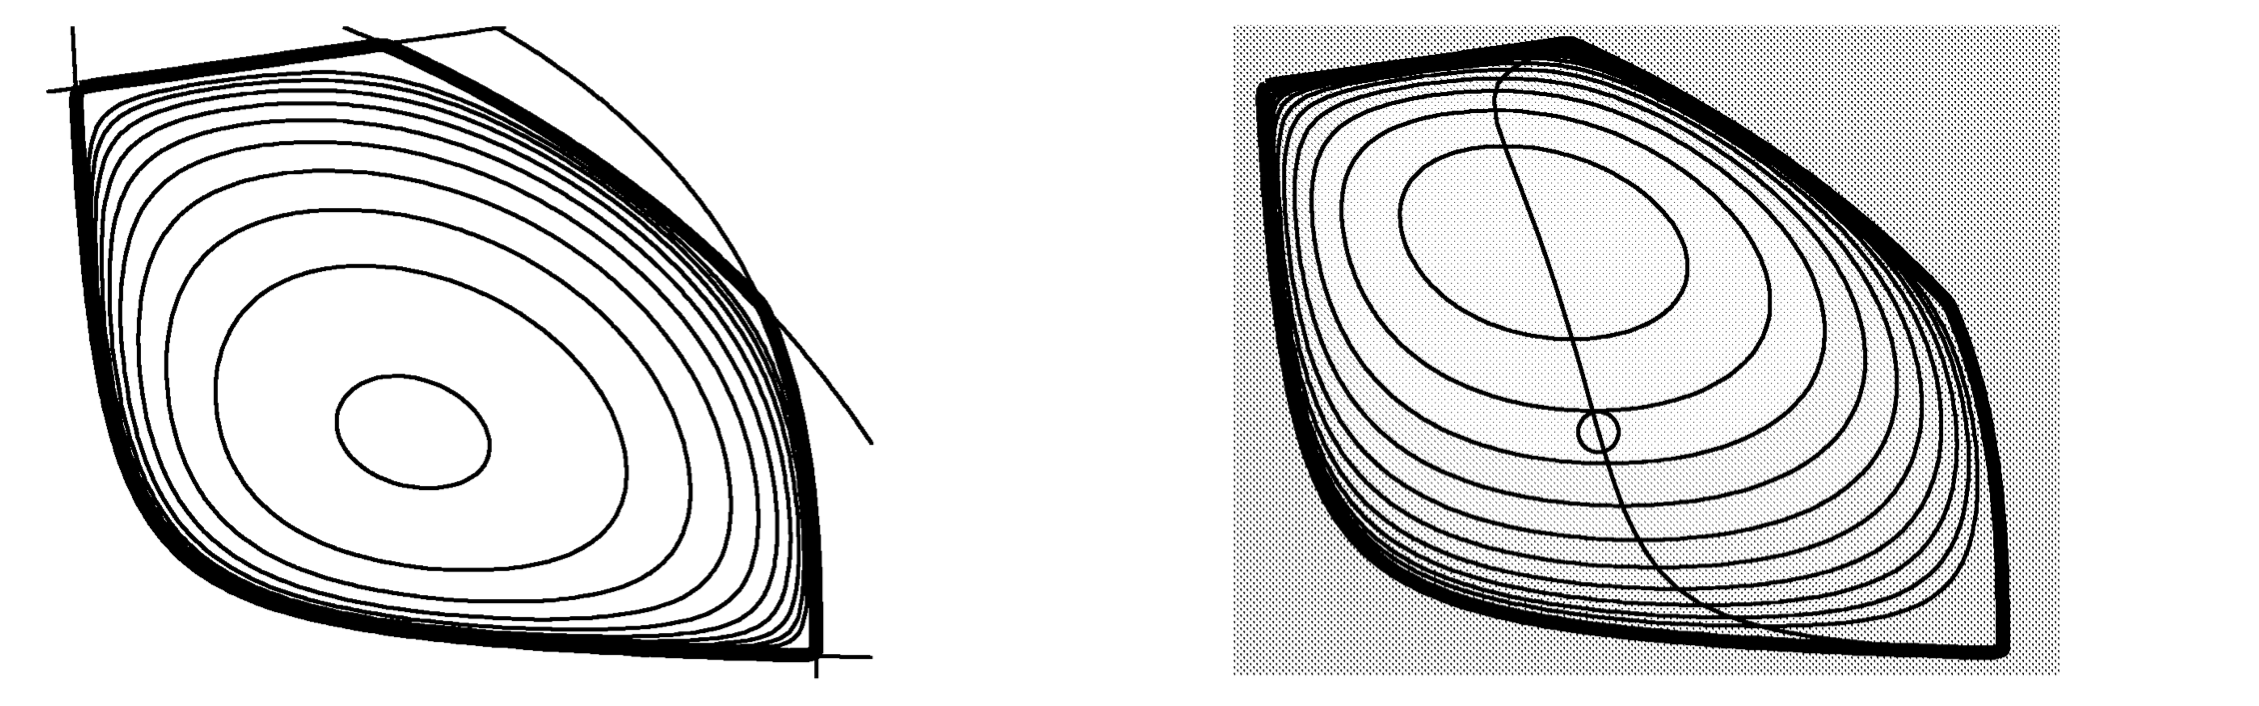
\includegraphics[width=.5\textwidth]{img/central_path.png}
\end{figure}
The optimum value $x_\mu^*$ of this problem tends to $x^*$ a solution of the original problem when $\mu$ decreases to zero, following the central path. 
\begin{itemize}
    \item [$\rightarrow$] Note: When $C$ is defined with convex constraints $g_i(x)\le 0$, we can use the barrier function $F(x)=-\sum_i\log(-g_i(x))$.
\end{itemize}
\subsection{Self-concordant barriers}
$F:int(C)\mapsto \R$ is called a $\nu$-self-concordant barrier for $C$ iff 
\begin{itemize}
    \item $F\in \mathcal{C}^3$ is convex;
    \item $F(x)\xrightarrow{x\rightarrow \partial C} +\infty$;
    \item The following two conditions hold:
    \begin{align}
        \nabla^3 F(x)[h,h,h]\le 2(\nabla F(x)[h,h])^{3/2}\\
        \nabla F(x)^T (\nabla F(x))^{-1}\nabla F(x)\le \nu\\
    \end{align}
    for all $x\in int(C)$ and $h\in \R^n$.
\end{itemize}
\subsubsection{Properties}
\begin{itemize}
    \item If $f$ is $\nu_1$-s.c. for $C_1$ and $G$ is $\nu_2$-s.c. for $C_2$, then $f+G$ is $(\nu_1+\nu_2)$-s.c. for $C_1\cap C_2$ (if nonempty);
    \item If $x\mapsto F(x)$ is a $\nu$-s.c. barrier for $C$, then $y\mapsto F(c-A^Ty)$ is a $\nu$-s.c. barrier for the set $\{y\text{ such that } c-A^Ty\in C\}$.
\end{itemize}
\subsection{Computing $x_\mu$}
By definition, 
\begin{equation}
    x_\mu = \arg_{x\in int(C)}\min \frac{c^Tx}{\mu}+F(x)
\end{equation}
and thus satisfies the condition 
\begin{equation}
    \frac{c}{\mu}+\nabla F(x)=0
\end{equation}
To compute $x_\mu$, we use Newton steps $n_\mu(x)$:
\begin{equation}
    n_\mu(x) = -\nabla^2f_\mu(x)\nabla f_\mu(x) = -\nabla^2F(x)(\frac{c}{\mu}+\nabla F(x))
\end{equation}
In practice, this method is not efficient, as it takes a long time to only compute a starting point. 
\begin{thm}
    Assume $x$ is such that $\delta_\mu(x)\le \tau<1$. Then, 
    \begin{equation}
        c^Tx - c^Tx^* < \frac{\nu \mu}{1-\tau}
    \end{equation}
\end{thm}
This means that choosing $\mu_{final}$ as the solution to $\frac{\nu\mu}{1-\tau}=\epsilon$ guarantees a final $\epsilon$ accuracy on the linear objective. 
\subsection{Short-step path-following method}
Given a starting iterate $x_0$ not too far from a point on the central path $x_0\approx x_{\mu_0}$, 
\begin{algorithm}[H]
    \caption{Short-step path-following method}\label{algo:sspf}
    \begin{algorithmic}[1]
        \State Find a $\nu$-s.c. barrier $F$ such that $dom(F)=int(C)$;
        \State Choose $0<\tau<1$ and $0<\theta<1$;
        \State Given a starting point $x_0\in int(C)$ and target accuracy $\epsilon$:
        \qquad \State Find initial value $\mu_0$ such that $\delta_{\mu_0}(x_0)\le \tau$;
        \qquad \State Compute final value $\mu_f=\epsilon \frac{1-\tau}{\nu}$;
        \qquad \State Set $k\leftarrow 0$, perform the main loop:
        \qquad \While{$\mu_k>\mu_f$}
        \State \qquad \textbf{Step 1:} $\mu_{k+1}\leftarrow \mu_k(1-\theta)$;
        \State \qquad \textbf{Step 2:} $x_{k+1}\leftarrow x_k+n_{\mu_{k+1}}(x_k)$;
        \State \qquad \textbf{Step 3:} $k\leftarrow k+1$;
        \EndWhile
    \end{algorithmic}
\end{algorithm}
This algorithm takes polynomial time. \\
As the distance to the central path is impossible to compute in practice, we approximate it to $\delta_{\mu_k}(x)=\lVert n_\mu(x)\rVert_x$.\\
This method reaches an accuracy $\epsilon$ on the objective within $\mathcal{O}\left(\sqrt{\nu}\log \frac{1}{\epsilon}\right)$ iterations. Therefore, it takes polynomial time if computing $F, \nabla F, \nabla^2 F$ takes polynomial time. 
\section{Practical details}
\begin{itemize}
    \item The barrier function is very hard to compute, but there exists universal ones for some specific domains (e.g. cones). 
\end{itemize}
\subsection{Initialisation procedure}
\begin{enumerate}
    \item Pick a reasonable starting iterate $\bar x$ that belongs to $int(C)$;
    \item Find a reasonable starting $\mu_0$:
    \begin{itemize}
        \item Any value $\mu_0>0$ works, but if too small, it will lead to longer initialization;
        \item $\mu_0=\min_{\mu} \delta_\mu(\bar x)$ works well. 
    \end{itemize}
    \item Compute $x_0$ by minimizing this problem starting from $\bar x$ and using damped Newton steps:
    \begin{equation}
        \min \frac{c^Tx}{\mu_0} + F(x)
    \end{equation}
    \item Stop the procedure when $\delta_{\mu_0}(x_0)\le \tau$.
\end{enumerate}

\end{document}